The examples below illustrate the use of the Simulink implementation above.

\begin{example}{bouncing ball with input}
\label{ex:bbinput} For the simulation of the bouncing ball system  with a constant input and regular data given by

\begin{eqnarray}
f(x,u):=\left[
 \begin{array}{c}
   x_{2} \\
 -\gamma
 \end{array}
\right],
   C : = \defset{ (x,u) \in \Re^{2}\times\Re}{x_{1} \geq u} \\
g(x,u):=\left[ \begin{array}{c}
 u \\
- \lambda x_{2}
\end{array}
\right]\ ,
    D: = \defset{ (x,u) \in \Re^{2}\times\Re}{x_{1} \leq u \ , \
  x_{2} \leq 0}
\end{eqnarray}
where $\gamma >0$ is the gravity constant, $u$ is the input constant,
and $\lambda \in [0,1)$ is the restitution coefficient.
The MATLAB scripts in each of the function blocks of the implementation above are given as follows.
An input was chosen to be $u(t,j) = 0.2$ for all $(t,j)$. The constants for the bouncing ball
system are $\gamma = 9.81$ and $\lambda=0.8$.

\bigskip

\noindent The following procedure is used to simulate this example using the model in the file {\tt Example\_1\_2a.slx}:
\begin{itemize}
\item {\tt Example\_1\_2a.slx} is opened in MATLAB/Simulink.
\item The {\em Embedded MATLAB function blocks} {\em f, C, g, D} are edited by double-clicking on the block and editing the script. In each embedded function block, parameters must be added as inputs and defined as parameters by selecting {\tt Tools>Edit Data/Ports}, and setting the scope to {\tt Parameter}. For this example, {\em gamma} and {\em lambda} are defined in this way.
\item The initialization script {\tt initialization.m} is edited by opening the file and editing the script. The flow time and jump horizons, $T$ and $J$ are defined as well as the initial conditions for the state vector, $x_0$, and input vector, $u_0$, and a rule for jumps, $rule$.
\item The postprocessing script {\tt postprocessing.m} is edited by opening the file and editing the script. Flows and jumps may be plotted by calling the functions {\em plotflows} and {\em plotjumps}, respectively. The hybrid arc may be plotted by calling the function {\em plotHybridArc}.
\item The simulation stop time and other simulation parameters are set to the values defined in {\tt initialization.m} by selecting {\tt Simulation>Configuration Parameters>Solver} and inputting $T$, $RelTol$, $MaxStep$, etc..
\item The masked integrator system is double-clicked and the simulation horizons and initial conditions are set as desired.
\item The block labeled {\em Double Click to Initialize} is double-clicked to initialize variables.
\item The simulation is run by clicking the run button or selecting {\tt Simulation>Start}.
\item The block labeled {\em Double Click to Plot Solutions} is double-clicked to plot the desired solutions.
\end{itemize}

%\begin{figure}[ht]
%  \begin{center}
%  \psfrag{flows [t]}[c]{flows [$t$]}
%  \psfrag{jumps [j]}[c]{jumps [$j$]}
%  \psfrag{x1}[c]{$x_1$}
%    {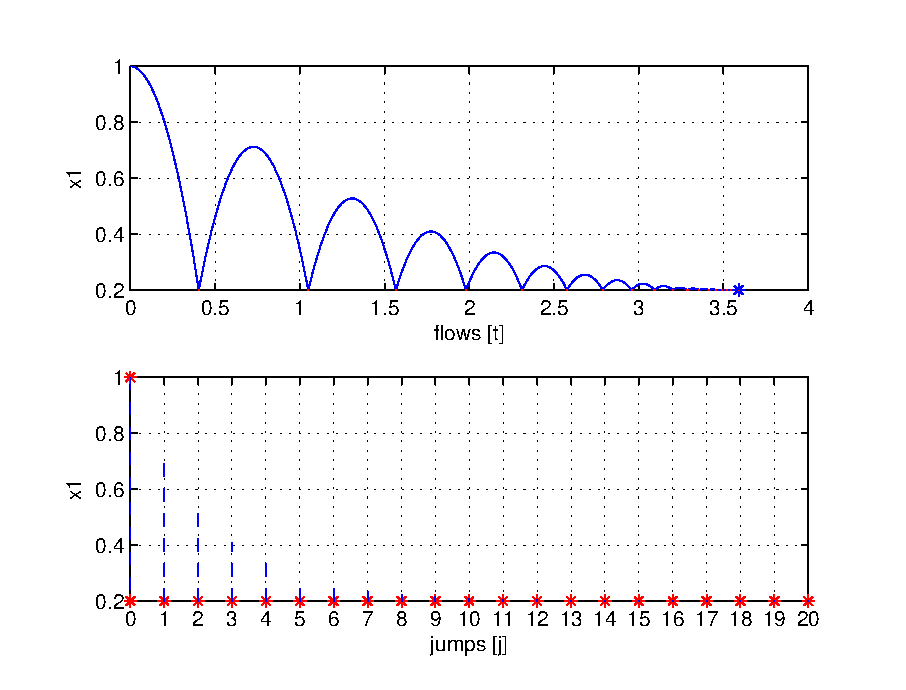
\includegraphics[width=.8\textwidth]{figures/Examples/FlowsAndJumps1.eps}}
%   \caption{Solution of Example~\ref{ex:bbinput}: height}
%\label{fig:input-1}
%  \end{center}
%\end{figure}
%
%\begin{figure}[ht]
%  \begin{center}
%  \psfrag{flows [t]}[c]{flows [$t$]}
%  \psfrag{jumps [j]}[c]{jumps [$j$]}
%  \psfrag{x2}[c]{$x_2$}
%    {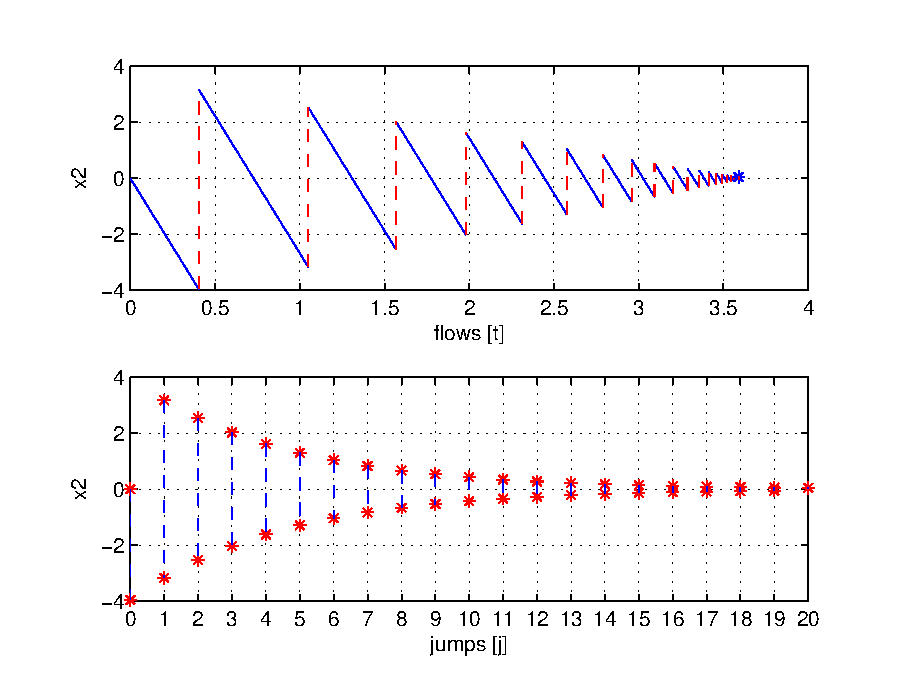
\includegraphics[width=.8\textwidth]{figures/Examples/FlowsAndJumps2.eps}}
%   \caption{Solution of Example~\ref{ex:bbinput}: velocity}
%\label{fig:input-2}
%  \end{center}
%\end{figure}

\begin{figure}[ht]
\begin{center}
\subfigure[Height \label{fig:input-1}]
{
\psfragfig[width=.45\textwidth]{figures/Examples/FlowsAndJumps1}
{
  \psfrag{flows [t]}[c]{flows [$t$]}
  \psfrag{jumps [j]}[c]{jumps [$j$]}
  \psfrag{x1}[c]{$x_1$}
  \psfrag{x2}[c]{$x_2$}
}
}
\qquad
\subfigure[Velocity \label{fig:input-2}]
{
    \psfragfig[width=.45\textwidth]{figures/Examples/FlowsAndJumps2}
{
  \psfrag{flows [t]}[c]{flows [$t$]}
  \psfrag{jumps [j]}[c]{jumps [$j$]}
  \psfrag{x1}[c]{$x_1$}
  \psfrag{x2}[c]{$x_2$}
}
}
\end{center}
\caption{Solution of Example~\ref{ex:bbinput}}
\end{figure}

\begin{figure}[ht]
  \begin{center}
  \psfrag{t}[c]{$t$}
  \psfrag{j}[c]{$j$}
  \psfrag{x1}[c]{$x_1$}
    {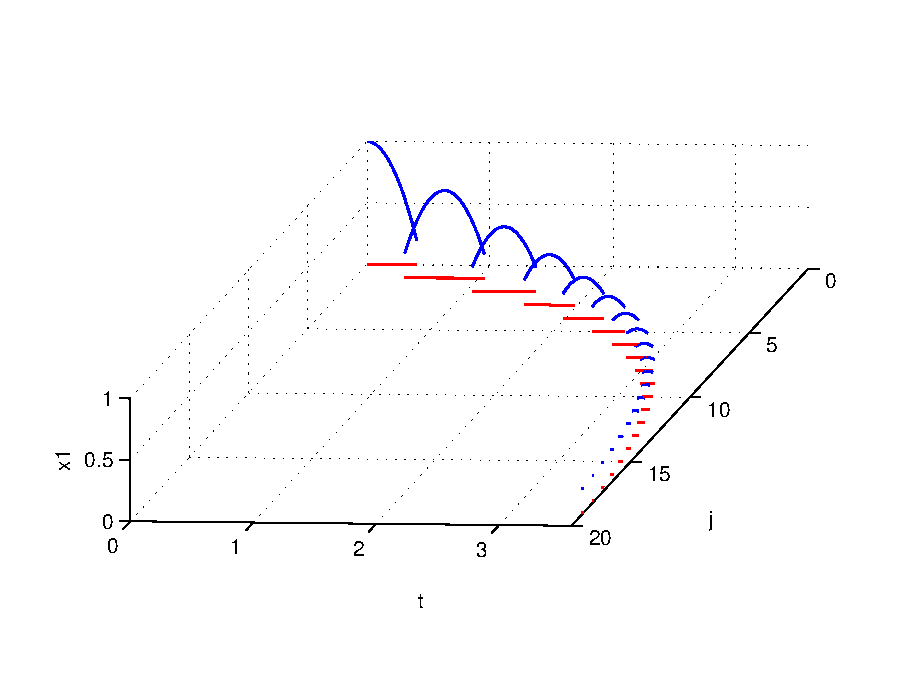
\includegraphics[width=.8\textwidth]{figures/Examples/HybridArc1.eps}}
   \caption{Hybrid arc corresponding to a solution of Example~\ref{ex:bbinput}: height}
  \end{center}
\end{figure}

% Set the location for MATLAB files included via the "\code" command.
\codeLocation{Matlab2tex_1_3}

\code{f.m}
\code{C.m}
\code{g.m}
\code{D.m}

% Flow map
% %\scriptsize
% % This file was automatically created from the m-file 
% "m2tex.m" written by USL. 
% The fontencoding in this file is UTF-8. 
%  
% You will need to include the following two packages in 
% your LaTeX-Main-File. 
%  
% \usepackage{color} 
% \usepackage{fancyvrb} 
%  
% It is advised to use the following option for Inputenc 
% \usepackage[utf8]{inputenc} 
%  
  
% definition of matlab colors: 
\definecolor{mblue}{rgb}{0,0,1} 
\definecolor{mgreen}{rgb}{0.13333,0.5451,0.13333} 
\definecolor{mred}{rgb}{0.62745,0.12549,0.94118} 
\definecolor{mgrey}{rgb}{0.5,0.5,0.5} 
\definecolor{mdarkgrey}{rgb}{0.25,0.25,0.25} 
  
\DefineShortVerb[fontfamily=courier,fontseries=m]{\$} 
\DefineShortVerb[fontfamily=courier,fontseries=b]{\#} 
  
\noindent                    
 \hspace*{-1.6em}{\scriptsize 1}$  $\color{mblue}$function$\color{black}$ xdot = f(x, u, gamma)$\\
 \hspace*{-1.6em}{\scriptsize 2}$  $\\
 \hspace*{-1.6em}{\scriptsize 3}$  $\color{mgreen}#%%%%%%%%%%%%%%%%%%%%%%%%%%%%%%%%%%%%%%%%%%%%%%%%%%%%%%%%%%%%%%%%%%%%%%%%%%%#\color{black}$$\\
 \hspace*{-1.6em}{\scriptsize 4}$  $\color{mgreen}$% Matlab Function  Author: Ricardo Sanfelice $\color{black}$$\\
 \hspace*{-1.6em}{\scriptsize 5}$  $\color{mgreen}$% (Revised by Giampiero Campa)$\color{black}$$\\
 \hspace*{-1.6em}{\scriptsize 6}$  $\color{mgreen}$% (Revised by Pablo Nanez)$\color{black}$$\\
 \hspace*{-1.6em}{\scriptsize 7}$  $\color{mgreen}$%$\color{black}$$\\
 \hspace*{-1.6em}{\scriptsize 8}$  $\color{mgreen}$% Project: Simulation of a hybrid system (Bouncing Ball)$\color{black}$$\\
 \hspace*{-1.6em}{\scriptsize 9}$  $\color{mgreen}$%$\color{black}$$\\
 \hspace*{-2em}{\scriptsize 10}$  $\color{mgreen}$% Name: f.m$\color{black}$$\\
 \hspace*{-2em}{\scriptsize 11}$  $\color{mgreen}$%$\color{black}$$\\
 \hspace*{-2em}{\scriptsize 12}$  $\color{mgreen}$% Description: Flow map$\color{black}$$\\
 \hspace*{-2em}{\scriptsize 13}$  $\color{mgreen}$%$\color{black}$$\\
 \hspace*{-2em}{\scriptsize 14}$  $\color{mgreen}$% Version: 1.0$\color{black}$$\\
 \hspace*{-2em}{\scriptsize 15}$  $\color{mgreen}$% Required files: - $\color{black}$$\\
 \hspace*{-2em}{\scriptsize 16}$  $\color{mgreen}#%%%%%%%%%%%%%%%%%%%%%%%%%%%%%%%%%%%%%%%%%%%%%%%%%%%%%%%%%%%%%%%%%%%%%%%%%%%#\color{black}$$\\
 \hspace*{-2em}{\scriptsize 17}$  $\\
 \hspace*{-2em}{\scriptsize 18}$  $\\
 \hspace*{-2em}{\scriptsize 19}$  $\color{mgreen}$% flow map: xdot=f(x,u);$\color{black}$$\\
 \hspace*{-2em}{\scriptsize 20}$  xdot = [x(2); gamma];$\\ 
  
\UndefineShortVerb{\$} 
\UndefineShortVerb{\#}\label{scr:f}
% %\normalsize

% Flow set
% %\scriptsize
% % This file was automatically created from the m-file 
% "m2tex.m" written by USL. 
% The fontencoding in this file is UTF-8. 
%  
% You will need to include the following two packages in 
% your LaTeX-Main-File. 
%  
% \usepackage{color} 
% \usepackage{fancyvrb} 
%  
% It is advised to use the following option for Inputenc 
% \usepackage[utf8]{inputenc} 
%  
  
% definition of matlab colors: 
\definecolor{mblue}{rgb}{0,0,1} 
\definecolor{mgreen}{rgb}{0.13333,0.5451,0.13333} 
\definecolor{mred}{rgb}{0.62745,0.12549,0.94118} 
\definecolor{mgrey}{rgb}{0.5,0.5,0.5} 
\definecolor{mdarkgrey}{rgb}{0.25,0.25,0.25} 
  
\DefineShortVerb[fontfamily=courier,fontseries=m]{\$} 
\DefineShortVerb[fontfamily=courier,fontseries=b]{\#} 
  
\noindent                          
 \hspace*{-1.6em}{\scriptsize 1}$  $\color{mblue}$function$\color{black}$ v  = C(x, u)$\\
 \hspace*{-1.6em}{\scriptsize 2}$  $\color{mgreen}$%--------------------------------------------------------------------------$\color{black}$$\\
 \hspace*{-1.6em}{\scriptsize 3}$  $\color{mgreen}$% Matlab M-file Project: HyEQ Toolbox @  Hybrid Systems Laboratory (HSL),$\color{black}$$\\
 \hspace*{-1.6em}{\scriptsize 4}$  $\color{mgreen}$% https://hybrid.soe.ucsc.edu/software$\color{black}$$\\
 \hspace*{-1.6em}{\scriptsize 5}$  $\color{mgreen}$% http://hybridsimulator.wordpress.com/$\color{black}$$\\
 \hspace*{-1.6em}{\scriptsize 6}$  $\color{mgreen}$%--------------------------------------------------------------------------$\color{black}$$\\
 \hspace*{-1.6em}{\scriptsize 7}$  $\color{mgreen}$% Project: Simulation of a hybrid system$\color{black}$$\\
 \hspace*{-1.6em}{\scriptsize 8}$  $\color{mgreen}$% Description: Flow set$\color{black}$$\\
 \hspace*{-1.6em}{\scriptsize 9}$  $\color{mgreen}$%--------------------------------------------------------------------------$\color{black}$$\\
 \hspace*{-2em}{\scriptsize 10}$  $\color{mgreen}$%--------------------------------------------------------------------------$\color{black}$$\\
 \hspace*{-2em}{\scriptsize 11}$  $\color{mgreen}$%   See also HYEQSOLVER, PLOTARC, PLOTARC3, PLOTFLOWS, PLOTHARC,$\color{black}$$\\
 \hspace*{-2em}{\scriptsize 12}$  $\color{mgreen}$%   PLOTHARCCOLOR, PLOTHARCCOLOR3D, PLOTHYBRIDARC, PLOTJUMPS.$\color{black}$$\\
 \hspace*{-2em}{\scriptsize 13}$  $\color{mgreen}$%   Copyright @ Hybrid Systems Laboratory (HSL),$\color{black}$$\\
 \hspace*{-2em}{\scriptsize 14}$  $\color{mgreen}$%   Revision: 0.0.0.3 Date: 05/20/2015 3:42:00$\color{black}$$\\
 \hspace*{-2em}{\scriptsize 15}$  $\color{mgreen}$%$\color{black}$$\\
 \hspace*{-2em}{\scriptsize 16}$  $\color{mgreen}$% Check on flow conditions$\color{black}$$\\
 \hspace*{-2em}{\scriptsize 17}$  $\color{mgreen}$% E.g.,$\color{black}$$\\
 \hspace*{-2em}{\scriptsize 18}$  $\color{mgreen}$% if (x(1) >= u(1))  % flow condition$\color{black}$$\\
 \hspace*{-2em}{\scriptsize 19}$  $\color{mgreen}$%     v = 1;  % report flow$\color{black}$$\\
 \hspace*{-2em}{\scriptsize 20}$  $\color{mgreen}$% else$\color{black}$$\\
 \hspace*{-2em}{\scriptsize 21}$  $\color{mgreen}$%     v = 0;   % do not report flow$\color{black}$$\\
 \hspace*{-2em}{\scriptsize 22}$  $\color{mgreen}$% end$\color{black}$$\\
 \hspace*{-2em}{\scriptsize 23}$  $\\
 \hspace*{-2em}{\scriptsize 24}$  $\\
 \hspace*{-2em}{\scriptsize 25}$  v = 1; $\color{mgreen}$% report flow$\color{black}$$\\
 \hspace*{-2em}{\scriptsize 26}$  $\\ 
  
\UndefineShortVerb{\$} 
\UndefineShortVerb{\#}\label{scr:C}
% %\normalsize

% Jump map
% %\scriptsize
% % This file was automatically created from the m-file 
% "m2tex.m" written by USL. 
% The fontencoding in this file is UTF-8. 
%  
% You will need to include the following two packages in 
% your LaTeX-Main-File. 
%  
% \usepackage{color} 
% \usepackage{fancyvrb} 
%  
% It is advised to use the following option for Inputenc 
% \usepackage[utf8]{inputenc} 
%  
  
% definition of matlab colors: 
\definecolor{mblue}{rgb}{0,0,1} 
\definecolor{mgreen}{rgb}{0.13333,0.5451,0.13333} 
\definecolor{mred}{rgb}{0.62745,0.12549,0.94118} 
\definecolor{mgrey}{rgb}{0.5,0.5,0.5} 
\definecolor{mdarkgrey}{rgb}{0.25,0.25,0.25} 
  
\DefineShortVerb[fontfamily=courier,fontseries=m]{\$} 
\DefineShortVerb[fontfamily=courier,fontseries=b]{\#} 
  
\noindent   
 \hspace*{-1.6em}{\scriptsize 1}$  $\color{mblue}$function$\color{black}$ xplus = g(x, u, lambda)$\\
 \hspace*{-1.6em}{\scriptsize 2}$  $\color{mgreen}$% jump map$\color{black}$$\\
 \hspace*{-1.6em}{\scriptsize 3}$  xplus = [u(1); -lambda*x(2)];$\\ 
  
\UndefineShortVerb{\$} 
\UndefineShortVerb{\#}\label{scr:g}
% %\normalsize

% Jump set
% %\scriptsize
% % This file was automatically created from the m-file 
% "m2tex.m" written by USL. 
% The fontencoding in this file is UTF-8. 
%  
% You will need to include the following two packages in 
% your LaTeX-Main-File. 
%  
% \usepackage{color} 
% \usepackage{fancyvrb} 
%  
% It is advised to use the following option for Inputenc 
% \usepackage[utf8]{inputenc} 
%  
  
% definition of matlab colors: 
\definecolor{mblue}{rgb}{0,0,1} 
\definecolor{mgreen}{rgb}{0.13333,0.5451,0.13333} 
\definecolor{mred}{rgb}{0.62745,0.12549,0.94118} 
\definecolor{mgrey}{rgb}{0.5,0.5,0.5} 
\definecolor{mdarkgrey}{rgb}{0.25,0.25,0.25} 
  
\DefineShortVerb[fontfamily=courier,fontseries=m]{\$} 
\DefineShortVerb[fontfamily=courier,fontseries=b]{\#} 
  
\noindent                         
 \hspace*{-1.6em}{\scriptsize 1}$  $\color{mblue}$function$\color{black}$ v  = D(x, u) $\\
 \hspace*{-1.6em}{\scriptsize 2}$  $\\
 \hspace*{-1.6em}{\scriptsize 3}$  $\color{mgreen}#%%%%%%%%%%%%%%%%%%%%%%%%%%%%%%%%%%%%%%%%%%%%%%%%%%%%%%%%%%%%%%%%%%%%%%%%%%%#\color{black}$$\\
 \hspace*{-1.6em}{\scriptsize 4}$  $\color{mgreen}$% Matlab Function  Author: Ricardo Sanfelice $\color{black}$$\\
 \hspace*{-1.6em}{\scriptsize 5}$  $\color{mgreen}$% (Revised by Giampiero Campa)$\color{black}$$\\
 \hspace*{-1.6em}{\scriptsize 6}$  $\color{mgreen}$% (Revised by Pablo Nanez)$\color{black}$$\\
 \hspace*{-1.6em}{\scriptsize 7}$  $\color{mgreen}$%$\color{black}$$\\
 \hspace*{-1.6em}{\scriptsize 8}$  $\color{mgreen}$% Project: Simulation of a hybrid system (Bouncing ball)$\color{black}$$\\
 \hspace*{-1.6em}{\scriptsize 9}$  $\color{mgreen}$%$\color{black}$$\\
 \hspace*{-2em}{\scriptsize 10}$  $\color{mgreen}$% Name: D.m$\color{black}$$\\
 \hspace*{-2em}{\scriptsize 11}$  $\color{mgreen}$%$\color{black}$$\\
 \hspace*{-2em}{\scriptsize 12}$  $\color{mgreen}$% Description: Jump set$\color{black}$$\\
 \hspace*{-2em}{\scriptsize 13}$  $\color{mgreen}$%$\color{black}$$\\
 \hspace*{-2em}{\scriptsize 14}$  $\color{mgreen}$% Version: 1.0$\color{black}$$\\
 \hspace*{-2em}{\scriptsize 15}$  $\color{mgreen}$% Required files: - $\color{black}$$\\
 \hspace*{-2em}{\scriptsize 16}$  $\color{mgreen}#%%%%%%%%%%%%%%%%%%%%%%%%%%%%%%%%%%%%%%%%%%%%%%%%%%%%%%%%%%%%%%%%%%%%%%%%%%%#\color{black}$$\\
 \hspace*{-2em}{\scriptsize 17}$  $\\
 \hspace*{-2em}{\scriptsize 18}$  xtemp = zeros(2,1);$\\
 \hspace*{-2em}{\scriptsize 19}$  xtemp = x;$\\
 \hspace*{-2em}{\scriptsize 20}$  $\\
 \hspace*{-2em}{\scriptsize 21}$  $\color{mblue}$if$\color{black}$ (xtemp(1) <= u(1)) && (xtemp(2) <= 0)  $\color{mgreen}$% jump condition$\color{black}$$\\
 \hspace*{-2em}{\scriptsize 22}$      v = 1;  $\color{mgreen}$% report jump$\color{black}$$\\
 \hspace*{-2em}{\scriptsize 23}$  $\color{mblue}$else$\color{black}$$\\
 \hspace*{-2em}{\scriptsize 24}$      v = 0;   $\color{mgreen}$% do not report jump$\color{black}$$\\
 \hspace*{-2em}{\scriptsize 25}$  $\color{mblue}$end$\color{black}$$\\ 
  
\UndefineShortVerb{\$} 
\UndefineShortVerb{\#}\label{scr:D}
% %\normalsize

A solution to the bouncing ball system from $x(0,0)=[1,0]^\top$ and with $T=10, J=20$, $rule =1$, is
depicted in Figure~\ref{fig:input-1} (height) and Figure~\ref{fig:input-2} (velocity).  Both the projection
onto $t$ and $j$ are shown. Figure~\ref{fig:input-3} depicts the corresponding hybrid arc for the position state.

These simulations reflect the expected behavior of the bouncing ball model. Note the only
difference between this example and the example of a bouncing ball without a constant input is that, in this example, the ball bounces on a platform at a height of the chosen input value $0.2$ rather than the ground at a value of $0$.

For MATLAB/Simulink files of this example, see Examples/Example\_1.2a.

\end{example}
